% Chapter 4
\chapter{Transmission Expansion Planning by Quantum Annealing} % Main chapter title
\label{Chapter4} % For referencing the chapter elsewhere, use \ref{Chapter1} 
\section{Statement of the problem}
\textit{Transmission expansion planning} (TEP)\,\cite{Neumann2020TransmissionFlows} is a \textit{mixed integer linear programming} (MILP) problem that aims at finding the optimal way to expand the capacity of an energy system by reducing the cost function. It decides how many transmission lines to build and where to connect them in order to satisfy the energy demand on a distributed energy system with a high share of renewable energy sources. There are other components apart from transmission lines such as generators or storages, but considering them imply an increment in the number of variables of the problem so that a quantum annealer cannot tackle the full problem. However, this reduction in complexity implies that the problem we are solving is not realistic, so we should consider it just as our starting point.\\\\
We can control the number of variables of the problem according to
\begin{itemize}
    \item \textbf{Number of nodes:} Clustering techniques allow us to fix the number of nodes of the problem so that towns of a given network are grouped acting as a single town.
    \item \textbf{Snapshots of time}: In expansion problems is common to consider hourly snapshots of time of one year, i.e., a total of 8760 snapshots but we can restrict the problem to a subset of snapshots.
    \item \textbf{Connectivity of transmission lines}: We can control the connectivity between nodes so that we do not allow a node the possibily of being fully connected with the rest of nodes.
    \item \textbf{Adding targets}: In this chapter we tackle a single target, i.e., the cost function -- investment and operational cost -- but there are other targets such as the increment of renewable energy sources in a given region or the reduction of the carbon footprint.
\end{itemize}
The TEP scales badly using classical algorithms\,\cite{Oertel2014ComplexityEvaluation} and, at the same time, energy system models are getting larger and more complex due to the integration of decentralized weather-dependent renewable energy sources, intermittent loads, sector coupling and the increase of storage components. Currently, the problem is often linearized or the scope and granularity of the model are reduced using clustering algorithms. For this reason, any computational time reduction will have substantial implications in closing the granularity gap between what the current models can solve and the desired resolution needed by energy system operators. Because of the maturity of quantum computers large TEP problems cannot be solved fully by a quantum annealer. For this reason, we require of hybrid methods\,\cite{Ding2019ImplementationDesign,Zhao2021HybridProgrammingb} to decompose large problems into a master problem which can be solved by a quantum annealer and a sub-problem for which cutting-edge classical algorithms are going to be applied.\\\\
There are two ways of formulating the transmission expansion problem. In one hand, the brownfield model considers the currents lines installed in a network $l_{i}^{1}$ among with a set of candidate lines $l_{i}^{0}$. On the other hand, the greenfield model considers a empty network and a set of candidate lines $l_{k} \equiv l_{k}^{0}$.
\begin{figure}[H]
  \begin{center}
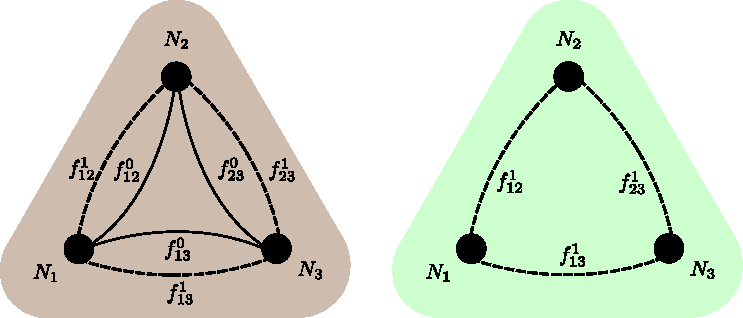
\includegraphics[width=0.9\textwidth]{Figures/3NodeBrownGreen.pdf}
  \end{center}
  \caption{Three node example. \textbf{Right:} Network considering current transmission lines and candidate lines, brownfield model. \textbf{Left:} Network considering just candidate lines, greenfield model.}
  \label{fig: ThreeNode}
\end{figure}
For simplicity, we are gonna consider the green grid approach so we do not have to take into account the constants associated with the installed lines. Notice each candidate lines connects two nodes, so that the variables could be written using two indexes $l_{ij}$ indicating that we are connecting node $i$ with node $j$. However, a QUBO problem works with single index variables, so we need a bijective mapping between two indexes $i,j$ to a single index $k$ for a given number of nodes $N$, see Ref.\,\cite{Jain2021SolvingComputer},
\begin{equation}
k(i,j,N) = \begin{cases}
    iN - i\left(i+1\right)/2 + j - (i+1), & i<j\\
    \text{None},& i=j \\
    k(j,i,N), & i>j
\end{cases}
    \label{eq: TwoIndexesmap}
\end{equation}
Hence, the cost function of our problem can be written as
\begin{equation}
\label{eq: Objective}
    \mathcal{H} = \underbrace{\sum_{k=1}^{L}c_{k}^{(\text{iv})}l_{k}}_{\text{Investment Cost}} + \underbrace{\sum_{t=1}^{T}\sum_{j=1}^{G}c_{j}^{(\text{oc})}g_{j}(t)}_{\text{Operational Cost}}\\ 
\end{equation}
subject to a set of linear constraints,
\begin{align}
    0 \leq g_{j,t}\leq g_{j}^{\max},\quad \forall j,t \\
    D_{i}(t) =\sum_{j=1}^{G}g_{j}(t), \quad \forall i,t \\
\end{align}
\begin{equation}
    \mathcal{H} = \sum_{k=1}^{L}c_{k}^{(\text{iv})}l_{k} + \sum_{t=1}^{T}\sum_{j=1}^{G}c_{j}^{(\text{oc})}g_{j}^{(\text{fixed})}(t) + P\left[\sum_{i}\sum_{t}\left(D_{i}(t) - \sum_{j=1}^{G}g_{j}^{(\text{fixed})}(t)l_{k(i,j,N)}\right)^{2}\right]
\end{equation}
The meaning of the variables is explained in the following table
\begin{table}[H]
\centering
\begin{tabular}{|c||c|c|} 
 \hline	
 \textbf{Symbol} & \textbf{Description} & \textbf{Type of variable} \\
 \hline	
 $N$ & Total number of nodes & Integer\\
  \hline	
 $L$ & Total number of candidate transmission lines & Integer\\
  \hline	
 $G$ & Total number of generators & Integer\\
  \hline	
 $T$ & Total number of snapshots & Integer\\
  \hline	
 $l_{k}$ & Candidate line with single-index $k$ & Binary\\
  \hline	
 $D_{i}(t)$ & Demand of node $i$ at snapshot $t$ & Real\\
  \hline	
 $g_{j}(t)$ & Energy production of generator $j$ at snapshot $t$ & Real\\
  \hline	
 $g_{j}^{(\text{max})}$ & Nominal power of generator $j$ & Real\\
  \hline	
 $c_{k}^{(\text{iv})}$ & Investment cost of line $k$ & Real\\
  \hline	
  $c_{j}^{(\text{oc})}$ & Annualised operational cost per MWh of generator $g_{j}$ & Real\\
  \hline
\end{tabular}
\caption{Description of variables involved in TEP problems}
\label{table:TEPNomenclature}
\end{table}
The investment cost $c_{k}^{(\text{iv})}$ is the cost of building the transmission line $l_{k}$ and it is a constant -- we are not considering time-dependent costs --, analogously, the operational cost $c_{j}^{(\text{oc})}$ represents the annualised cost per [MWh] of the produced energy $g_{j}(t)$ at time $t$. For simplicity, we set the operational cost to each carrier -- wind turbine, solar or run of river among others -- to a fixed value -- mean cost of that carrier -- so that we do not have to consider the variation of the cost as function of the node.\\\\
Notice, that the total cost depends on the investment cost and the operational cost. As stated before the number of possible configurations of our problem scale badly. For this reason, knowing if we are considering a large set of snapshots -- large investment planning - or just a tiny subset of snapshots gives us clues about what region of the configuration space we should explore. There are two regions to be considered,
\begin{itemize}
    \item \textbf{Large expansion planning:} Consider we are given a 10 year expansion planning problem, then if we produce the energy with the  cheapest carriers -- e.g. wind turbines -- we will reduce the operational cost drastically as compared with producing the energy with other carriers. Maybe the fact of producing the energy with the cheapest carriers implies we build the more expensive transmission lines, hence increasing the investment cost.
    \item \textbf{Short expansion planning:} Consider a single-snapshot, then it is obvious that the minimum total cost function imply a minimum in the investment cost regardeless of the operational cost, since the operational cost are lower as compared with the investment cost and only have one snapshot to act.
\end{itemize}
This trade-off between investment cost and operational cost is what determine the minimum value of the total cost function.\\\\
To summarise, we receive as input a given energy demand for a set of nodes $i$ for a set of snapshots $t$, then we optimise the network so that we build the minimum amount of transmission lines -- minimizing in that way the investment cost -- so that the energy demand is satisfied for each snapshot. We are also taking into account the operational cost of each carrier so there is a trade-off between the investment cost of transmission lines and the operational cost of generators used to produce the energy to satisfy the demand.
%%%%%%%%%%
\section{QUBO formulation of three-node TEP}
We start by considering a small network of three nodes $N=3$ with 3 existing lines $l_{k}^{(0)}\in \mathcal{L}^{(0)}$ and 3 candidate lines $l_{i}^{(1)}\in \mathcal{L}^{(1)}$, (Figure \ref{fig: ThreeNode}). The nodes can be though as towns whose energy demand has to be fulfilled and the lines allow the network to transmit energy between nodes so that if some node is producing more energy than its demand, then that excess of energy can be transmitted to other node of the network. For now we are going to focus on the ability of each node in transmitting energy to other node assuming a set of snapshots is given, i.e., in each snapshot a node will require energy from the other two nodes. Our task is to fulfill this energy transmission demand between nodes so that our investment cost is minimum.

Finally the QUBO matrix of this problem is,
\begin{equation}
Q =
        \begin{bmatrix}
           3T^{2} & 6T^{2} & 6T^{2} & 2T & 4T & 2T & 2T & 4T & 8T &2T & 4T & 8T  \\
           0 &3T^{2}& 6T^{2} & 2T & 4T & 2T & 2T & 4T & 8T &2T & 4T & 8T \\
           0 & 0 & 3T^{2} &2T & 4T & 2T & 2T & 4T & 8T &2T & 4T & 8T \\
           0 & 0 & 0 & 1 & 4 & 4 & 0 & 0 & 0 & 0 & 0 & 0\\
           0 & 0 & 0 & 0 & 4 & 8 & 0 & 0 & 0 & 0 & 0 & 0\\
           0 & 0 & 0 & 0 & 0 & 4 & 0 & 0 & 0 & 0 & 0 & 0\\
           0 & 0 & 0 & 0 & 0 & 0 & 1 & 4 & 8 & 0 & 0 & 0\\
           0 & 0 & 0 & 0 & 0 & 0 & 0 & 4 & 16& 0 & 0 & 0\\
           0 & 0 & 0 & 0 & 0 & 0 & 0 & 0 & 16& 0 & 0 & 0\\
           0 & 0 & 0 & 0 & 0 & 0 & 0 & 0 & 0 & 1 & 4 & 8 \\
           0 & 0 & 0 & 0 & 0 & 0 & 0 & 0 & 0 & 0 & 4 & 16\\
           0 & 0 & 0 & 0 & 0 & 0 & 0 & 0 & 0 & 0 & 0 & 16
         \end{bmatrix}
\end{equation}
\section{Running QUBO problem on D-WAVE's annealer}
\subsection{Three-Node without discretization in transmission capacities}
In this example we solved the three-node network with three candidate lines where the transmission capacities are fixed, i.e., if a line transmit electricity it does it always with the same value. In this way we can simplify the problem by not using slack variables for discretizing the transmisssion capacities.
%%%%%%%%%%%%%%%%%%%%%%%%%%%%%%%%%%%%%%%%%%%%%%%%%%%%%%%%%%%%%%%%%%%%%%%%%%%%%
% Hybrid Classical-Quantum annealing
%%%%%%%%%%%%%%%%%%%%%%%%%%%%%%%%%%%%%%%%%%%%%%%%%%%%%%%%%%%%%%%%%%%%%%%%%%%%%


D-Wave\,\cite{D-WaveDocumentation} allows us to formulate the QUBO by hand and use the  solver .... or we can .... using CQM ....

%%%%%%%%%%%%%%%%%%%%%%%%%%%%%%%%%%%%%%%%%%%%%%%%%%%%%%%%%%%%%%%%%%%%%%%%%%%%%%%
% IDEA PARA LA SECCION DE INVESTIGACION - PROPUESTA DE MEJORA DE PROTOCOLO
%%%%%%%%%%%%%%%%%%%%%%%%%%%%%%%%%%%%%%%%%%%%%%%%%%%%%%%%%%%%%%%%%%%%%%%%%%%%%%%
\section{Proposed protocols}
\subsection{QA-SA Heuristic Protocol}
In the original protocol a random criterion of selection is assigned to the neighboring function. However, this function can be optimised for a given problem by changing the selection criterion accordingly. For instance, for a large expansion planning the operational cost of a generator -- the annualised cost per $MWh$ of a carrier (wind energy, solar energy, gas, among others) --  is the terms that contribute the most to our total cost function. Because of this we can decide to generate neighboring configuration such that we start by building those generators with less operational cost. This criterion could also considers the number of snapshots and differences of operational cost with respect the investment planning of each generator and decide according to that. Furthermore, our problem has real constraints which implies it is not a good idea to solve the sub-problem(s) with the quantum annealer. For this reason, we reverse the original protocol so that the quantum annealer tackle the master problem and the classical solver tackle the sub-problem(s).
\begin{figure}[H]
\centering
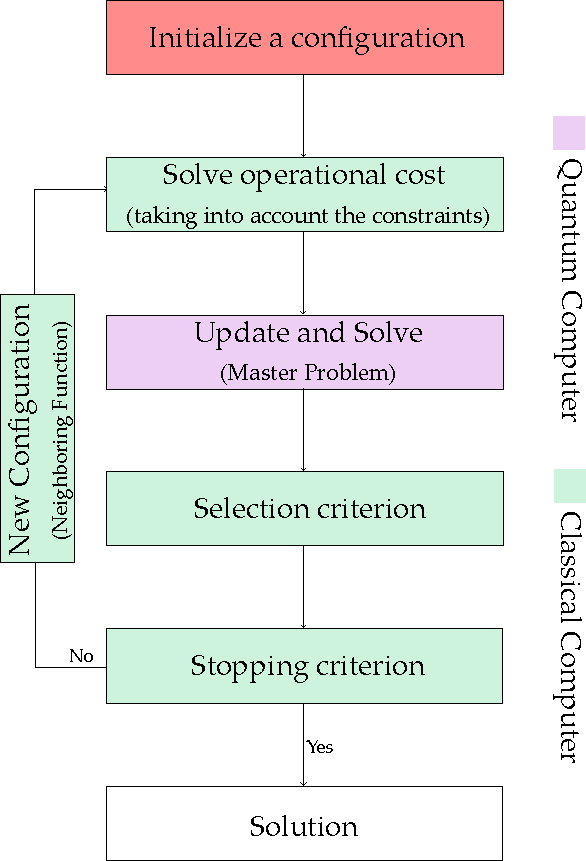
\includegraphics[width=0.5\textwidth]{Figures/QASAProtocol_Layer 1.pdf} 
\caption{QA-SA protocol scheme.}
\label{fig:QA_SAProtocol}
\end{figure}
\begin{enumerate}
    \item Set the cost to a high value and initialize a configuration for the problem.
    \item Solve the operational cost taking into account the constraints,
    \begin{align}
        \min  \sum_{j}c^{\text{iv}}_{j}l_{j} + \sum_{j}c_{j}^{(\text{oc})}g_{j} ,\quad \text{Subject to:}\\
        D_{k}(t) = \sum_{j}g_{j}, \quad \forall\, k,t \\
        0\leq g_{j} \leq g_{j}^{(max)}, \quad \forall\, j\\
        0 \leq l_{i} \leq l_{i}^{max}
    \end{align}
    \item Update the master problem with the generator $\{g_{j}\}$ value 
    \begin{equation}
        \sum_{j}c_{j}^{(\text{oc})}g_{j}^{(\text{fixed})}
    \end{equation}
    and introduce a penalty if the line connecting node $k$ with generators $g_{j}$ is not built
    \begin{equation}
        P\left[D_{k}(t) - \sum_{j}g_{j}^{(\text{fixed})}l_{j,k}\right]^{2}
    \end{equation}
    \item Apply the selection criterion to keep or to discard the current configuration.
    \item If stopping criterion is satisfied, then outputs the solution. Otherwise, generate a new configuration for $g_{j}$ and repeat steps 2 to 4.
\end{enumerate}